
\documentclass[10pt,A4]{article}	

\usepackage[utf8]{inputenc}		

\usepackage{xstring, xifthen}

\usepackage[default]{raleway}

\renewcommand*\familydefault{\sfdefault} 	
\usepackage[T1]{fontenc}

\usepackage{moresize}

\usepackage{fontawesome}

\newcommand{\vcenteredinclude}[1]{\begingroup
\setbox0=\hbox{\includegraphics{#1}}%
\parbox{\wd0}{\box0}\endgroup}

\newcommand*{\vcenteredhbox}[1]{\begingroup
\setbox0=\hbox{#1}\parbox{\wd0}{\box0}\endgroup}

\newcommand{\icon}[3] { 							
	\makebox(#2, #2){\textcolor{maincol}{\csname fa#1\endcsname}}
}	

\newcommand{\icontext}[4]{ 						
	\vcenteredhbox{\icon{#1}{#2}{#3}}  \hspace{2pt}  \parbox{0.9\mpwidth}{\textcolor{#4}{#3}}
}

\newcommand{\iconhref}[5]{ 						
    \vcenteredhbox{\icon{#1}{#2}{#5}}  \hspace{2pt} \href{#4}{\textcolor{#5}{#3}}
}

\newcommand{\iconemail}[5]{ 						
    \vcenteredhbox{\icon{#1}{#2}{#5}}  \hspace{2pt} \href{mailto:#4}{\textcolor{#5}{#3}}
}

\usepackage{paracol}

\usepackage[a4paper]{geometry}

\geometry{top=1cm, bottom=1cm, left=1cm, right=1cm}

\usepackage{fancyhdr}
\pagestyle{empty}

\setlength{\parindent}{0mm}

\usepackage{array}

\newcolumntype{x}[1]{%
>{\raggedleft\hspace{0pt}}p{#1}}%

\usepackage{graphicx}
		
\usepackage{tikz}				
\usetikzlibrary{shapes, backgrounds,mindmap, trees}

\usepackage{transparent}
\usepackage{color}

\definecolor{maincol}{RGB}{ 225, 0, 0 }

\definecolor{darkcol}{RGB}{ 70, 70, 70 }

\definecolor{lightcol}{RGB}{245,245,245}

\usepackage[hidelinks]{hyperref}

\newcommand{\mpwidth}{\linewidth-\fboxsep-\fboxsep}

\newcommand{\cvlist}[1] {
	\begin{itemize}{#1}\end{itemize}
}

\newcommand{\cvtext}[1] {
	\begin{tabular*}{1\mpwidth}{p{0.98\mpwidth}}
		\parbox{1\mpwidth}{#1}
	\end{tabular*}
}

\newcommand{\cvsection}[1] {
	\vspace{14pt}
	\cvtext{
		\textbf{\LARGE{\textcolor{darkcol}{\uppercase{#1}}}}\\[-4pt]
		\textcolor{maincol}{ \rule{0.1\textwidth}{2pt} } \\
	}
}

\newcommand{\cvskill}[3] {
	\begin{tabular*}{1\mpwidth}{p{0.72\mpwidth}  r}
 		\textcolor{black}{\textbf{#1}} & \textcolor{maincol}{#2}\\
	\end{tabular*}
	
	\hspace{4pt}
	\begin{tikzpicture}[scale=1,rounded corners=2pt,very thin]
		\fill [lightcol] (0,0) rectangle (1\mpwidth, 0.15);
		\fill [maincol] (0,0) rectangle (#3\mpwidth, 0.15);
  	\end{tikzpicture}
}

\newcommand{\cvevent}[7] {

	\parbox{\mpwidth}{
		\begin{tabular*}{1\mpwidth}{p{0.72\mpwidth}  r}
	 		\textcolor{black}{\textbf{#2}} & \colorbox{maincol}{\makebox[0.25\mpwidth]{\textcolor{white}{#1}}} \\
			\textcolor{maincol}{\textbf{#3}} & \\
		\end{tabular*}\\[8pt]
	
		\ifthenelse{\isempty{#4}}{}{
			\cvtext{#4}\\
		}
	}

	\ifthenelse{\isempty{#5}}{}{
		\vspace{9pt}
		{#5}
	}
	
	\vspace{14pt}
}

\newcommand{\cvmetaevent}[4] {
	\textcolor{maincol} {\cvtext{\textbf{\begin{flushleft}#1\end{flushleft}}}}

	\ifthenelse{\isempty{#2}}{}{
	\textcolor{darkcol} {\cvtext{\textbf{#2}} }
	}

	\ifthenelse{\isempty{#3}}{}{
		\cvtext{{ \textcolor{darkcol} {#3} }}\\
	}

	\cvtext{#4}\\[14pt]
}

\newcommand{\cvqrcode}[1] {
	\begin{center}
		\includegraphics[width={#1}\mpwidth]{qrcode}
	\end{center}
}

\begin{document}
\columnratio{0.31}
\setlength{\columnsep}{2.2em}
\setlength{\columnseprule}{4pt}
\colseprulecolor{lightcol}
\begin{paracol}{2}
\begin{leftcolumn}

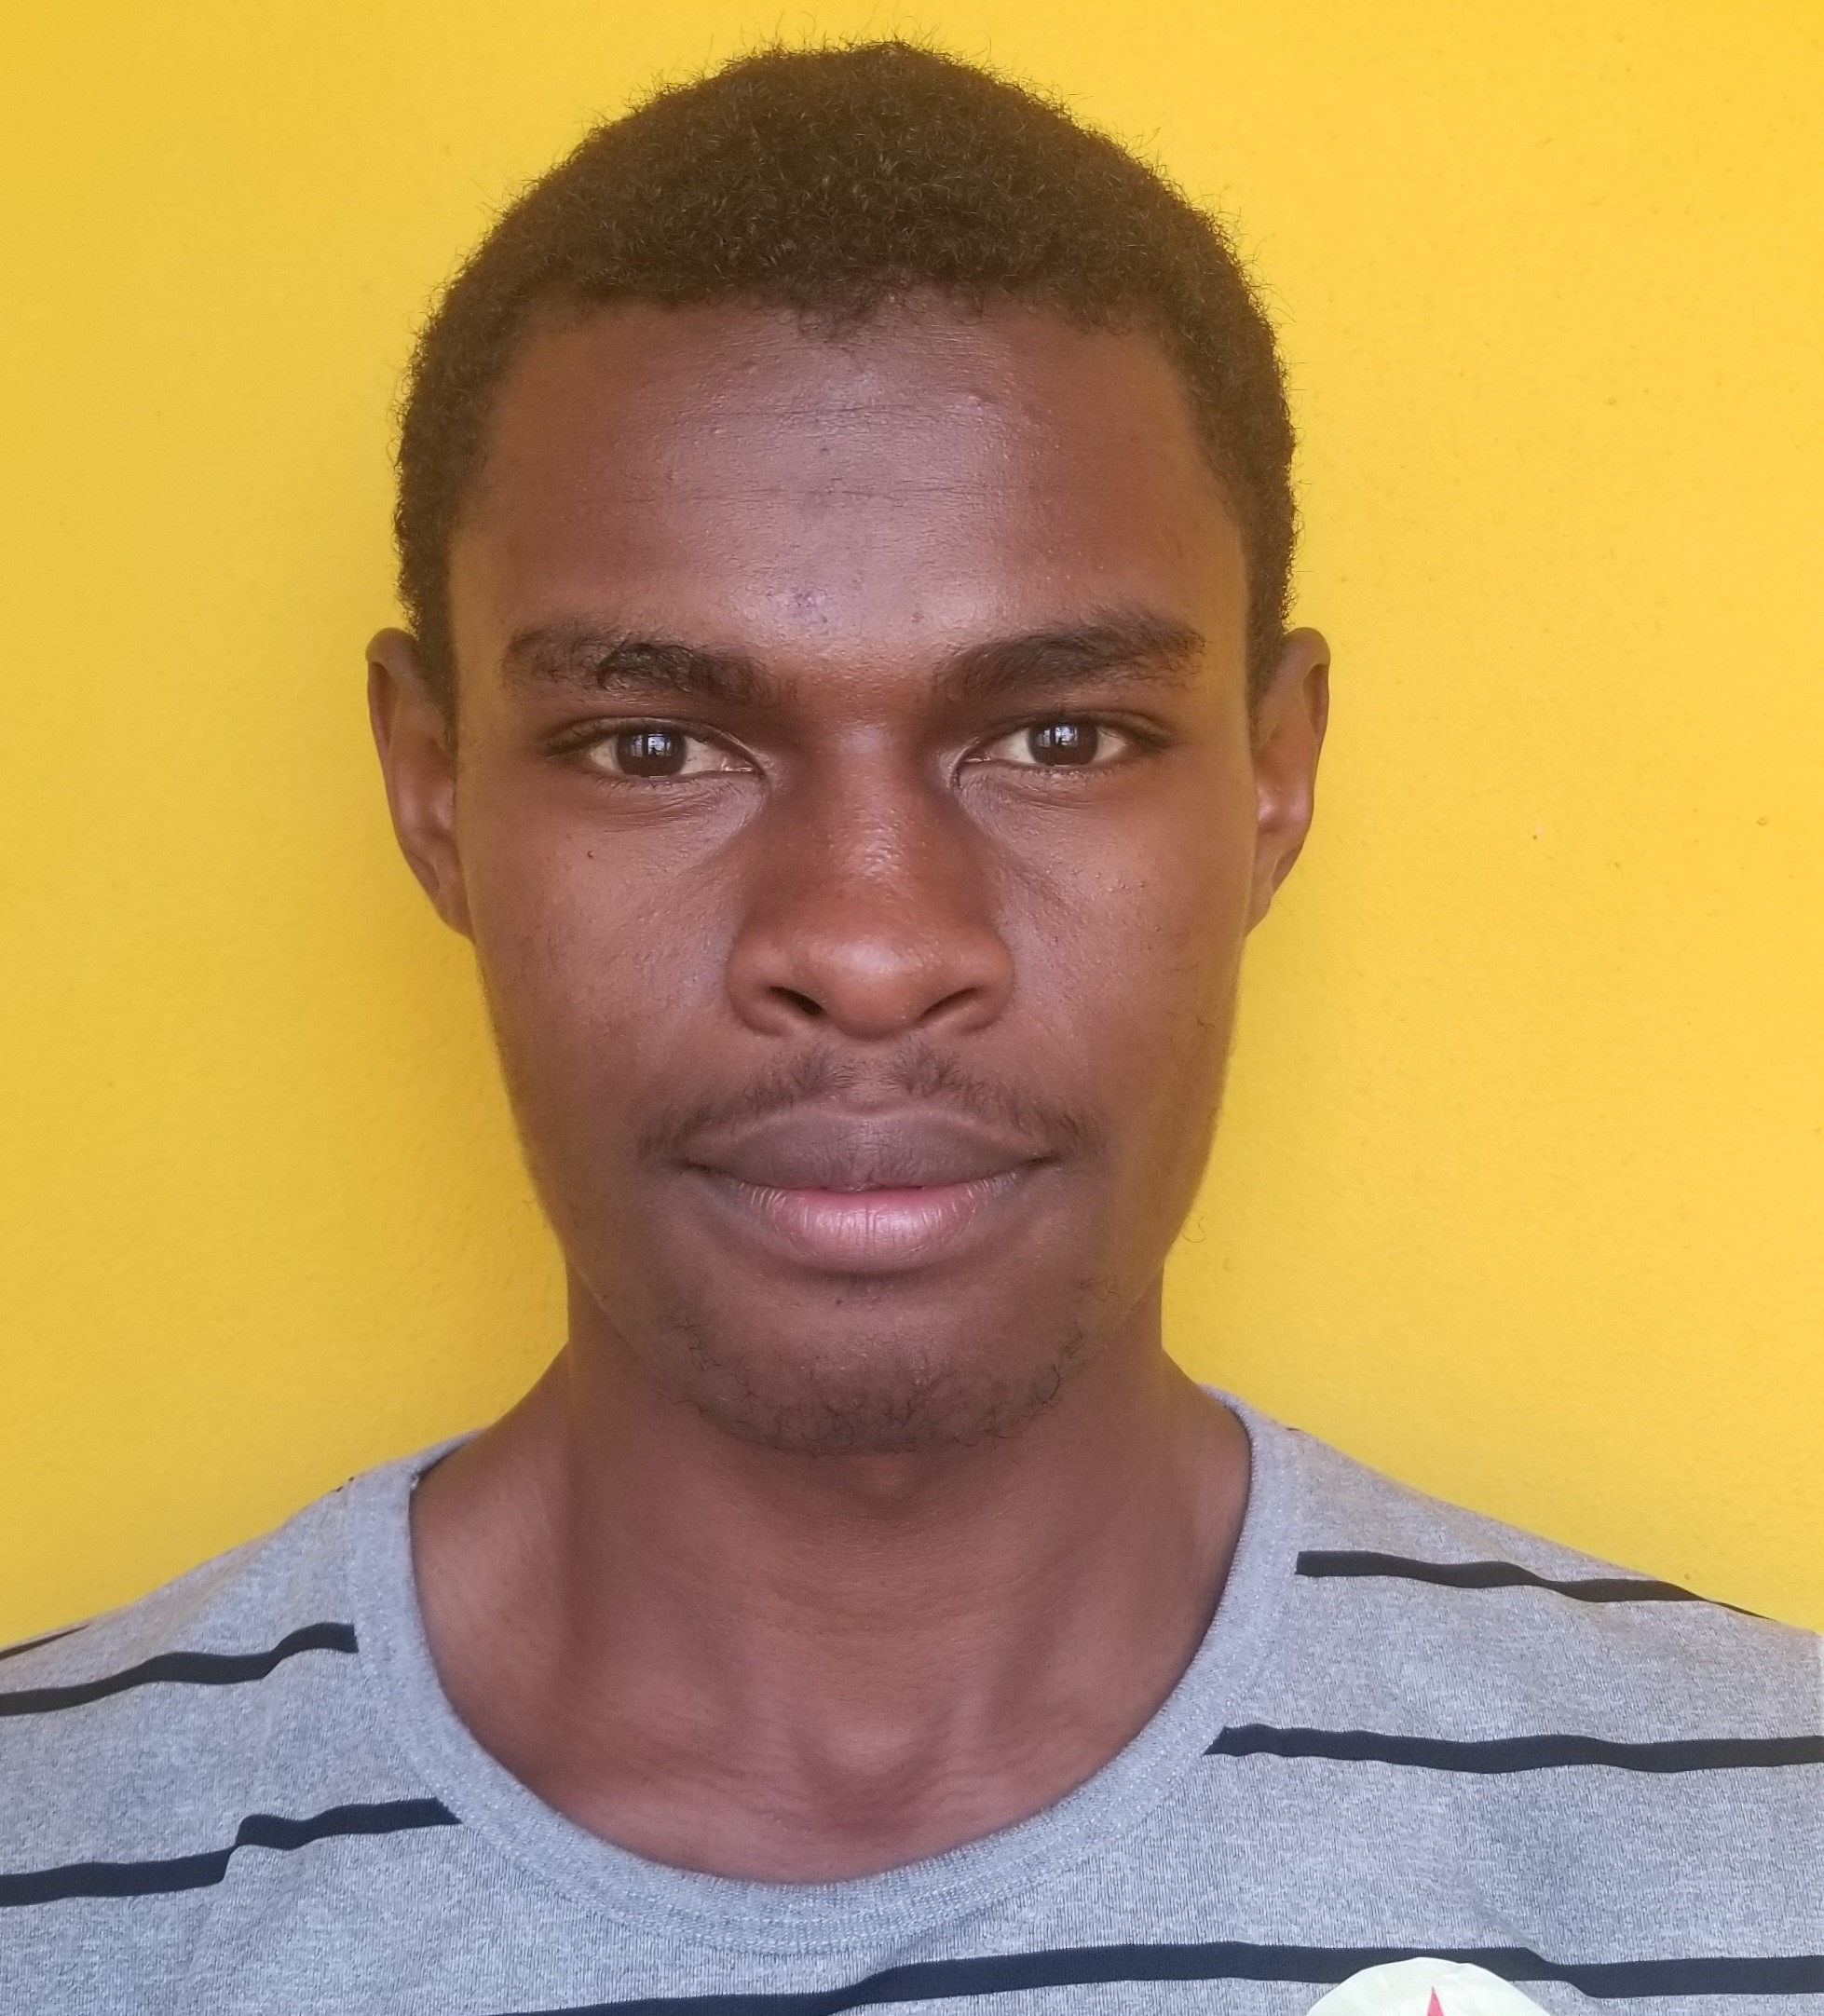
\includegraphics[width=\linewidth]{untitled.jpg}	

\cvsection{COMP\' ETENCES}

\cvskill{Windows/Linux} {+1 Ans} {1} \\[-2pt]

\cvskill{Python} {+1 Ans} {1} \\[-2pt]

\cvskill{Html/CSS/JS} {+1 Ans} {1} \\[-2pt]

\cvskill{PHP/MySQL} {7 Mois} {0.7} \\[-2pt]

\cvskill{GIT} {+6 Mois} {0.6} \\[-2pt]

\cvskill{C/C++/\texttt{C\#}} {+3 Mois} {0.3} \\[-2pt]

\cvskill{LaTex} {-1 Mois} {0.1} \\[-2pt]

\cvsection{CONTACT}
	
\icontext{MapMarker}{12}{Antananarive\\ 3D Ters S Antanimena}{black}\\[6pt]
\icontext{MobilePhone}{12}{+261 38 72 657 05 }{black}\\[6pt]
\iconemail{Envelope}{12}{raharison.tsidiany@esti.mg}{raharison.tsidiany@esti.mg}{black}\\[6pt]
\verb| |\faGithubSquare \quad devsuccess.github.io \\[6pt]

\cvqrcode{0.6}

\end{leftcolumn}
\begin{rightcolumn}

\fcolorbox{white}{darkcol}{\begin{minipage}[c][3.5cm][c]{1\mpwidth}
	\begin {center}
		\HUGE{ \textbf{ \textcolor{white}{ \uppercase{ TSIDIANY Raharison Muriel } } } } \\[-24pt]
		\textcolor{white}{ \rule{0.1\textwidth}{1.25pt} } \\[4pt]
		\large{ \textcolor{white} {Développeur Informatique} }
	\end {center}
\end{minipage}} \\[14pt]
\vspace{-12pt}

\vfill\null
\cvsection{PROFILE}

\cvtext{Je suis un jeune développeur informatique qui étudie actuellement à l'\' Ecole Supérieur des Technologies d'Information en licence 1. J'ai eu mon Bacc série D en 2021 à LPEF Sirama-Ambilobe.\\

Je me considère comme une personne sérieuse, plus d'une années d'expérience dans le cadre pratique et théorique de la programmation informatique, qui a pour passion le développement
de logiciels et application informatique que ce soit sur une plateforme web, mobile, lourde ou léger.\\
}


\cvsection{EXP\' ERIENCE PROFESSIONNEL}

\cvevent
	{Sept 2019 - 2021}
	{Président de l'Association Alpha LPEF}
	{A propos}
	{Alpha LPEF est une association à but non lucratif qui rassemble l'ensemble des étudiants du Lycée Privé d'Expression Français (LPEF), notre activité se traduit par des différentes activités sportives et de compétition interclasse, et des différentes activités extra-scolaires telle que des aides au pauvre\dots, j'était en charge de : }
	{\cvlist{
		\item Promouvoir la dynamique de groupe.
		\item Responsable premier de l'association vis-à-vis de l'école.
		\item Recherche des différentes donateurs\dots
	}}

\vfill
\cvsection{HOBBIES}
\cvevent
	{SPORT}
	{}
	{}
	{J'aime seulement le :}
	{\cvlist{
		\item Basquet-ball.
	}}


\cvevent
	{REPORTAGE}
	{}
	{}
	{J'aime plus les reportages concernant la téchnologie et découverte:}
	{\cvlist{
		\item Réver le futur.
		\item Tour du Monde.
	}}

\mbox{}
\mbox{}
\mbox{}
\mbox{}
\end{rightcolumn}
\end{paracol}
\end{document}

